\chapter{Разработка и создание испытательного стенда для измерения реактивных моментов}\label{ch:ch3}

В предыдущих главах были рассмотрены причины возникновения реактивных моментов при повороте оси визирования оптической системы КА. Математическое моделирование и экспериментальная отработка в космосе показали, что полностью учесть все факторы только расчётными методами невозможно. На практике проявляются дополнительные эффекты: люфты и неточности сборки редукторов, упругие деформации узлов крепления, дисбаланс маховиков, неравномерность распределения массы зеркал. Эти факторы приводят к появлению остаточных моментов и резонансных частот, которые трудно заранее оценить аналитически.

Таким образом, расчётных методов недостаточно для полной оценки динамики формирования реактивных моментов. Практика создания и эксплуатации космических оптико-механических систем показывает, что обязательным этапом юстировки аппаратуры является проведение наземных экспериментальных исследований, позволяющих:

\begin{itemize}
	\item проверить адекватность математических моделей;
	\item уточнить значения моментов инерции подвижных узлов;
	\item определить величины остаточных моментов, не поддающихся точному расчёту;
	\item разработать методы балансировки и оптимизации алгоритмов управления приводами.
\end{itemize}
	
Для решения этих задач необходим специализированный измерительный комплекс. В качестве такого комплекса был разработан испытательный стенд, позволяющий рассматривать исследуемую оптическую систему как колебательное звено, откликающееся на приложенный реактивный момент. В результате анализа угловых колебаний рамы стенда с закреплённой аппаратурой удаётся получить количественную оценку некомпенсированных реактивных моментов.

\section{Теоретическая модель стенда}

Разработанный стенд для измерения остаточных реактивных моментов основан на принципе представления исследуемой оптико-механической системы в виде колебательного звена. Подобная постановка позволяет использовать методы динамики твёрдого тела и теории малых колебаний для регистрации и анализа реактивных воздействий.

Динамика стенда описывается уравнением движения:

\begin{equation}
	\label{eq:stadeq}
	J\cdot \frac{d^2\varphi}{dt^2}+b \cdot \frac{d\varphi}{dt}+ c \cdot \varphi = M(t)
\end{equation}

где \(J\) --- момент инерции рамы вместе с установленной оптической системой, \(\varphi\) --- угол поворота рамы относительно равновесного положения, \(b\) --- коэффициент затухания, \(с\) --- коэффициент крутильной жёсткости, \(M(t)\) --- реактивный момент.

В удобной для анализа форме уравнения записывается как:

\begin{equation}
	\label{eq:standeq2}
	\ddot{\varphi}(t) + 2\,\xi\,\omega_0\,\dot{\varphi}(t) + \omega_0^{2}\,\varphi(t)
	= \frac{M(t)}{J}
\end{equation}

где \(\omega_0\) --- собственная частота колебательного звена, \(\xi\) --- декремент затухания.

ЛАЧХ колебательного звена показано на рисунке ~\cref{fig:afc}.

\begin{figure}[!h] 
	\centerfloat{
		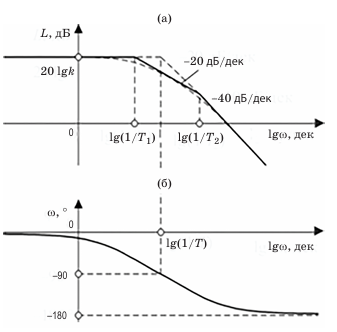
\includegraphics[scale=0.8]{afc} 
	}
	\caption{Логарифмическая амплитудная -а) и логарифмическая фазовая -б) частотные характеристики колебательного звена}
	\label{fig:afc} 
\end{figure}

Для корректного воспроизведения динамики необходимо, чтобы собственная частота маятника была смещена относительно диапазона характерных частот воздействия. В данном случае стенд спроектирован таким образом, что возмущающее воздействие проявляется в послерезонансной области. В этом случае колебательное звено работает как механический фильтр низких частот, подавляющий высокочастотные вибрации основания и внешние помехи, при этом сохраняется информативность основной составляющей измеряемого момента.

Моделирование стенда показало, что при увеличении декремента затухания выше $\xi=0,1$ форма выходного сигнала сильно искажается: снижается амплитуда и появляется фазовый сдвиг относительно входного воздействия (рисунок ~\cref{fig:decrement}). Поэтому при проектировании подвеса использовались материалы и схемы крепления, обеспечивающие малый уровень диссипативных потерь и обеспечивающие $\xi \leq 0,1$

\begin{figure}[!h]
	\centering
	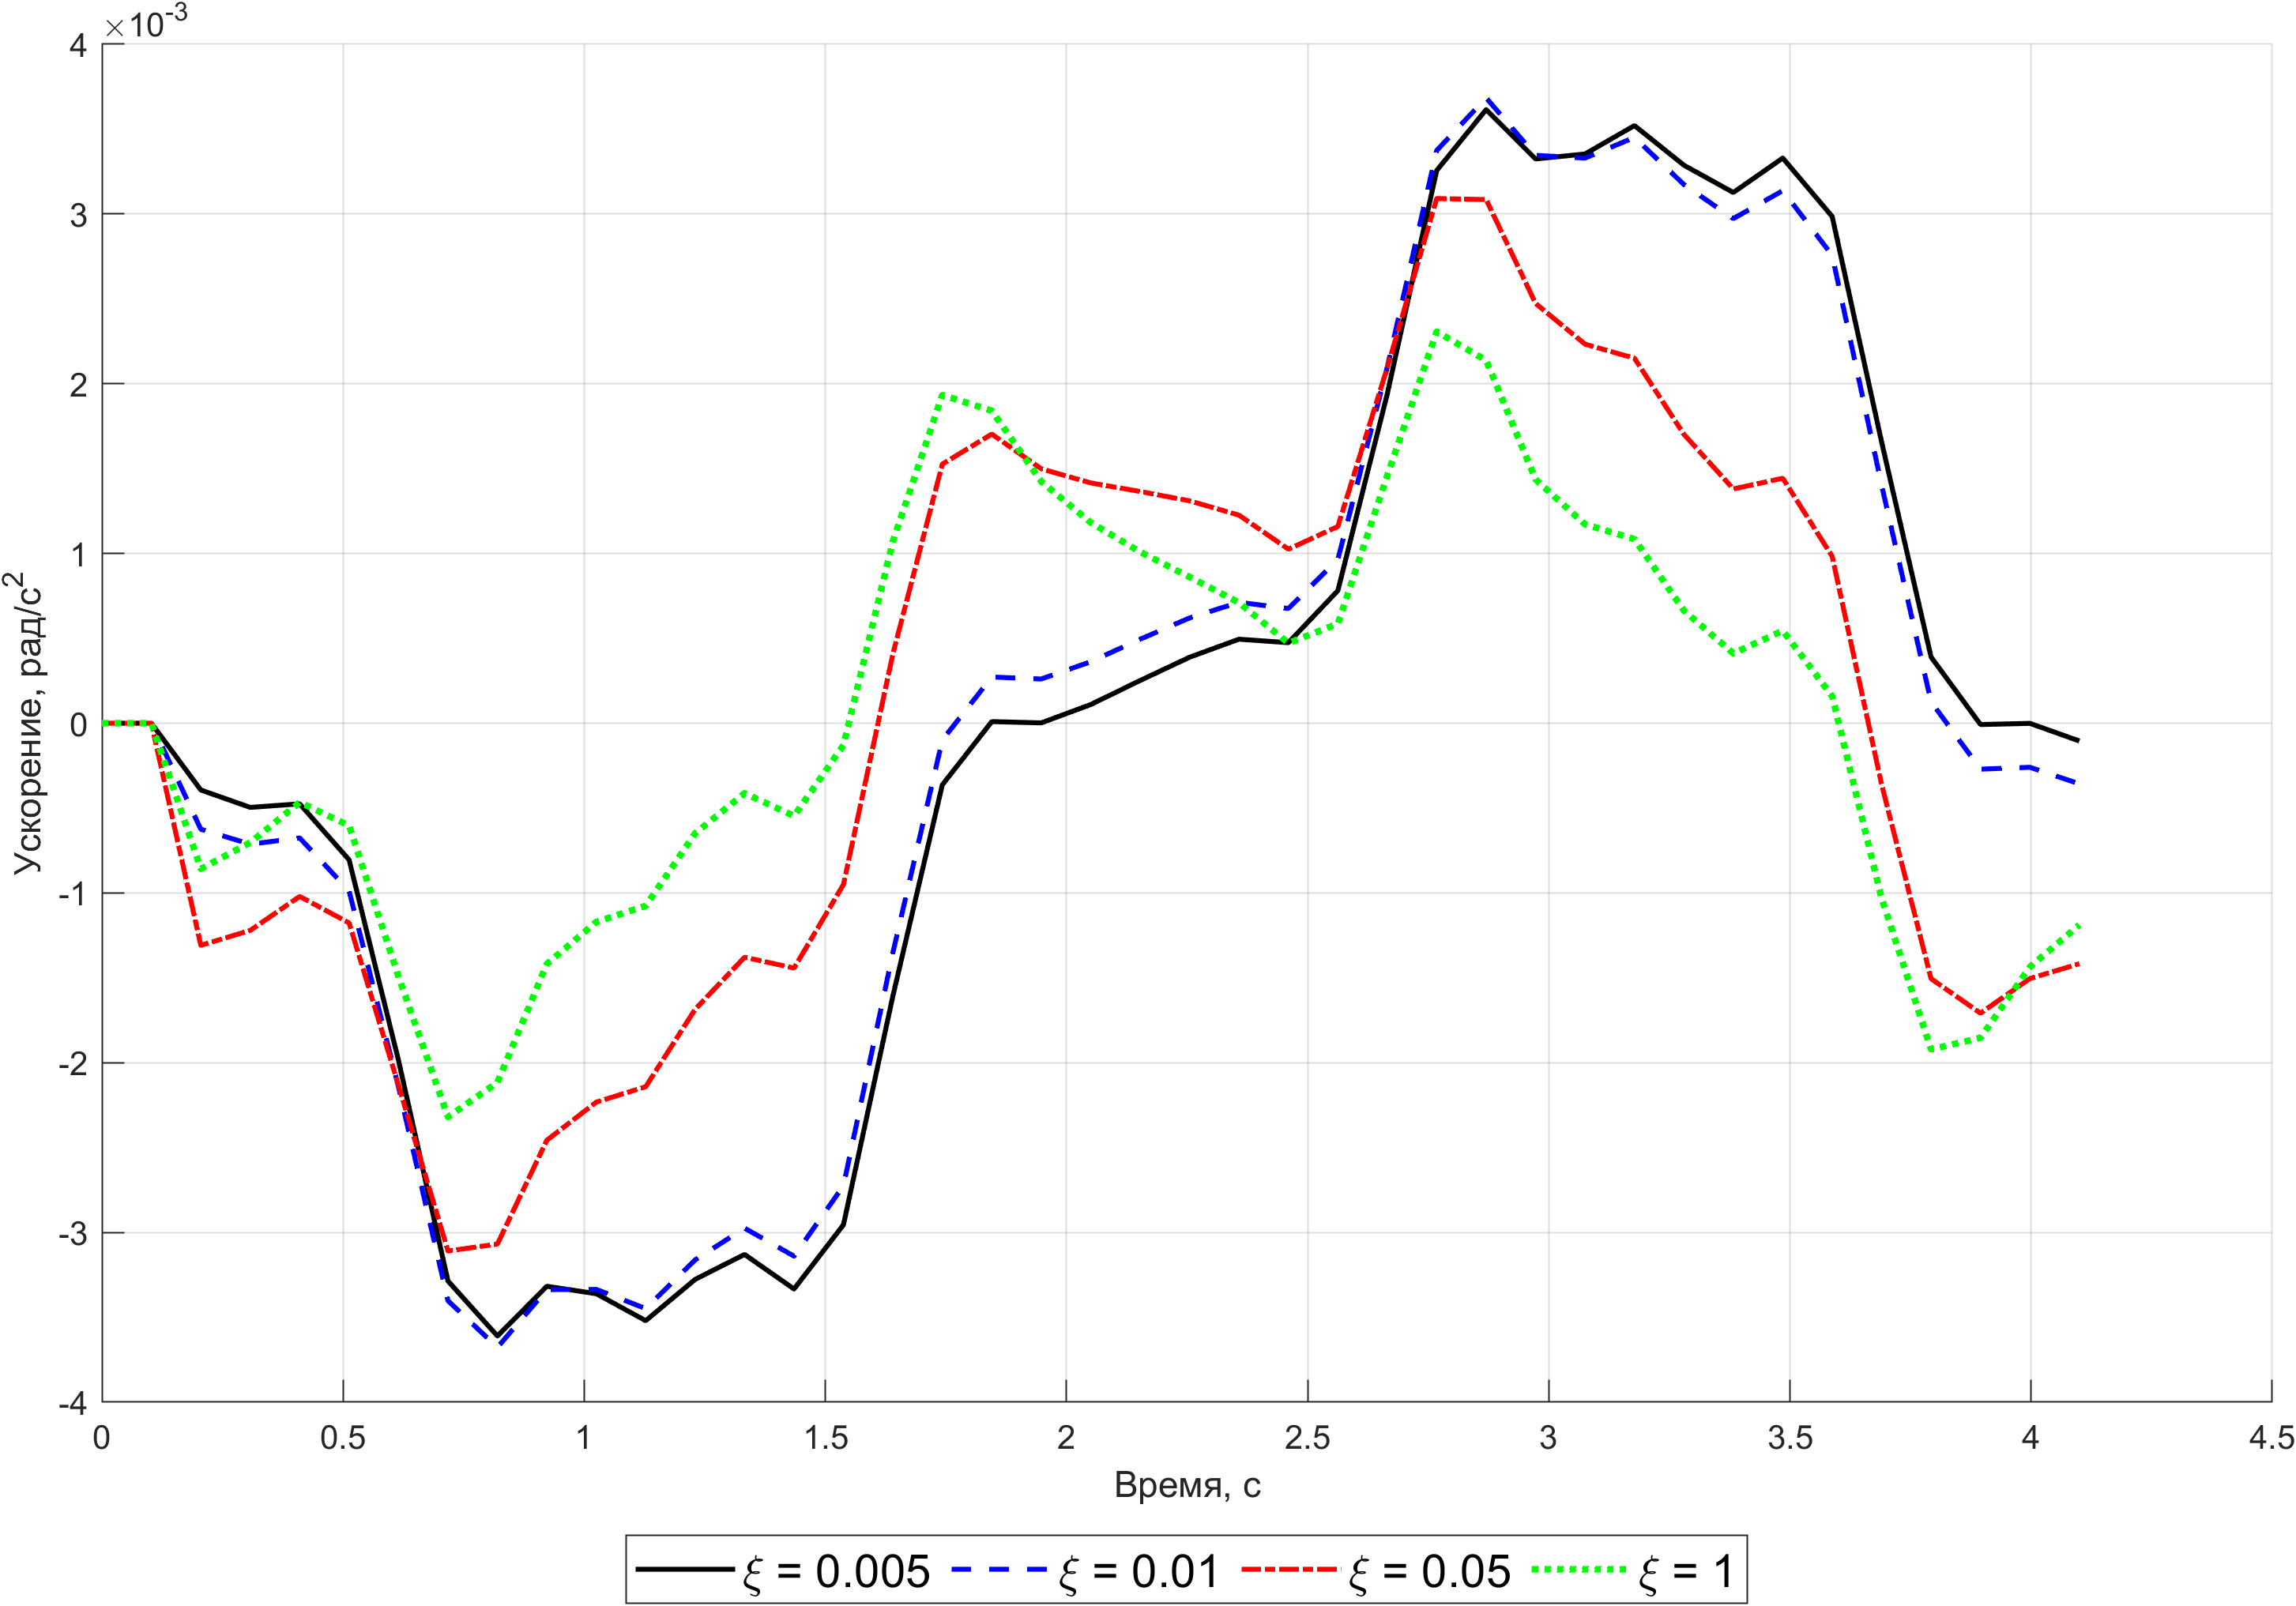
\includegraphics[scale=0.7]{matlab/decrement.png}
	\caption{Ускорение рамы с различными декрементами затухания}
	\label{fig:decrement}
\end{figure}

Таким образом, выбор параметра узла подвеса позволяет:

\begin{itemize}
	\item сместить собственную частоту колебаний стенда в область, лежащую ниже характерных частот рабочего воздействия;
	\item сохранить линейность отклика и минимизировать фазовые искажения;
	\item обеспечить режим работы стенда как фильтра, выделяющего динамику реактивного момент и подавляющего паразитные колебания.
\end{itemize}

\section{Конструктивное устройство стенда}

Конструктивно стенд представляет собой подвесную систему, обеспечивающую исследуемой ОМС одну степень свободы. Основой конструкции служит металлическая рама, подвешенная на металлической струне, выполняющей роль упругого элемента. Использование струны позволяет практически полностью исключить сухое трение. Внутри рамы располагается исследуемая оптическая система, закреплённая в изделиедержателе, представляющем собой металлический куб. Для возможности измерений по различным осям изделиедержатель может устанавливаться внутри рамы в разных ориентациях. Это позволяет без изменения конструкции стенда задавать требуемое направление измерений и исследовать динамику реактивных моментов по трём ортогональным осям.

Для обеспечения корректной работы подвесной системы необходимо исключить статический дисбаланс. Это достигается совмещением оси подвеса с центром масс нагрузки. Для этой цели используется регулируемый зацеп, позволяющий перемещать точку крепления струны в горизонтальной плоскости. Процесс юстировки выполняется с применением пузырькового уровня. 

В состав стенда входят волоконно-оптический гироскоп и тестовый маховик. Гироскоп закреплен на подвесной раме и регистрирует скорость её колебания. Тестовый маховик с известным моментом инерции служит для формирования контролируемого момента, воздействующего на стенд. Общий вид стенда приведён на рисунке ~\cref{fig:yoiom}

\begin{figure}[!h] 
	\centerfloat{
		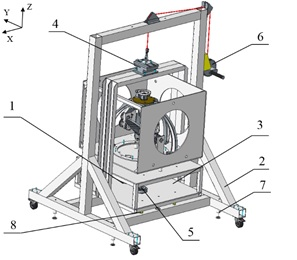
\includegraphics[scale=1.2]{yoiom} 
	}
	\legend{1 – маховик; 2 – рама; 3 – измерительная платформа; 4 – зацеп настраиваемый; 5 – волоконно-оптический гироскоп; 6 – лебёдка ручная; 7 – опоры-домкарты; 8 – конус}
	\caption{Стенд измерения реактивного момента}
	\label{fig:yoiom} 
\end{figure}

\section{Методика измерения реактивного момента}

\subsection{Принцип метода измерений}

Методика предназначена для измерения некомпенсированного реактивного момента, возникающего при перемещении подвижных частей оптико-механической системы (ОМС). Диапазон измерений охватывает значения от $10^{-3}$ до $1 \,\text{Н}\cdot\text{м}$.

Применяемый метод относится к категории косвенных. Измерение некомпенсированного момента выполняется через регистрацию скорости колебаний подвесной системы, вызванных реактивным воздействием. Регистрация осуществляется волоконно-оптическим гироскопом, установленным на подвижной раме. Для формирования эталонного воздействия используется тестовый маховик с заранее известным моментом инерции, установленный на отдельном приводе.

Суть метода заключается в сравнении ускорений колебаний подвеса, вызванных реактивным моментом оптико-механической системы, сравнивается с ускорением, возникающим при воздействии тестового маховика. Поскольку момент инерции подвеса в обоих случаях одинаковый, ускорение однозначно определяет величину приложенного момента. 



\subsection{Подготовка к проведению измерений}

Перед началом экспериментов исследуемая оптико-механическая система устанавливается в изделиедержатель стенда и фиксируется на фланце металлического куба. Далее выполняется юстировка подвесной системы. Для этой цели используется регулируемый зацеп, позволяющий смещать точку крепления струны в горизонтальной плоскости. Совмещение оси подвеса с центром масс подвижной части проводится по показаниям пузырькового уровня. После установки и юстировки производится подключение средств измерений и вспомогательного оборудования (см. Таблицу ~\cref{tab:equipment}). Включение аппаратуры выполняется заблаговременно, не менее чем за 30 минут до начала измерений, что необходимо для термостабилизации гироскопа и электронной части измерительной системы.

В обязательном порядке проверяется работоспособность волоконно-оптического гироскопа. Для этого прибор фиксируется на неподвижном основании и регистрирует проекцию угловой скорости вращения Земли. Измеренное значение сравнивается с расчётным, определяемым по географической широте места проведения эксперимента. Допустимое расхождение не должно превышать 0,3 \%, что подтверждает пригодность гироскопа к дальнейшему использованию. %todo subsubsection

%todo график гироскопа

Непосредственно перед измерениями контролируются условия окружающей среды. Температура воздуха в помещении должна находиться в пределах 15–35 °С, относительная влажность — 45–80 \%, атмосферное давление — 84–107 кПа. Контроль осуществляется с помощью барометра-анероида и психрометра. Соблюдение указанных параметров исключает влияние климатических факторов на точность эксперимента. Необходимые условия измерений представлены в Таблицу ~\cref{tab:conditions}

\subsection{Определение тестового момента}

Для задания \textcolor{yellow}{эталонного} воздействия на подвес используется тестовый маховик, установленный на отдельном приводе. Его момент инерции $J_m$ определяется один раз при сборке стенда на основе геометрических размеров и массы маховика. Измерения выполняются с использованием аттестованных средств измерений (штангенциркуля и весов), что гарантирует соответствие требованиям метрологического контроля. Подробный расчёт момента инерции приведён в приложении ~\ref{app:flyweel_inertia}

При подаче напряжения на двигатель, маховик начинает вращение по заданному закону изменения угловой скорости. Управляющая система обеспечивает трапецеидальный профиль разгона, что позволяет выделить участок равномерного ускорения. Профиль разгона показан на рисунке ~\cref{fig:flyweel_speed}.

\begin{figure}[!h] 
	\centerfloat{
	%	\includegraphics[scale=1.2]{matlab/img/flyweel_speed.pdf} 
	}
	\caption{Профиль разгона тестового маховика}
	\label{fig:flyweel_speed} 
\end{figure}



Скорость вращения определяется с помощью преобразователя угловых перемещений ЛИР-ДА190К. Угловая скорость определяется как отношение поворота маховика на угол $2\pi$ радиан к интервалу времени между двумя последовательными импульсами $t_{i+1}, t_i$ преобразователя: 

\begin{equation}
	\label{eq:flyweel_spd}
	\omega_i=\frac{2 \pi}{(t_{i+1}-t_i)}
\end{equation}

где \(i=1...5\) --- номер импульса.

Осциллограмма сигнала преобразователя представлена на рисунке ~\cref{fig:encoder}


\begin{figure}[!h] 
	\centerfloat{
		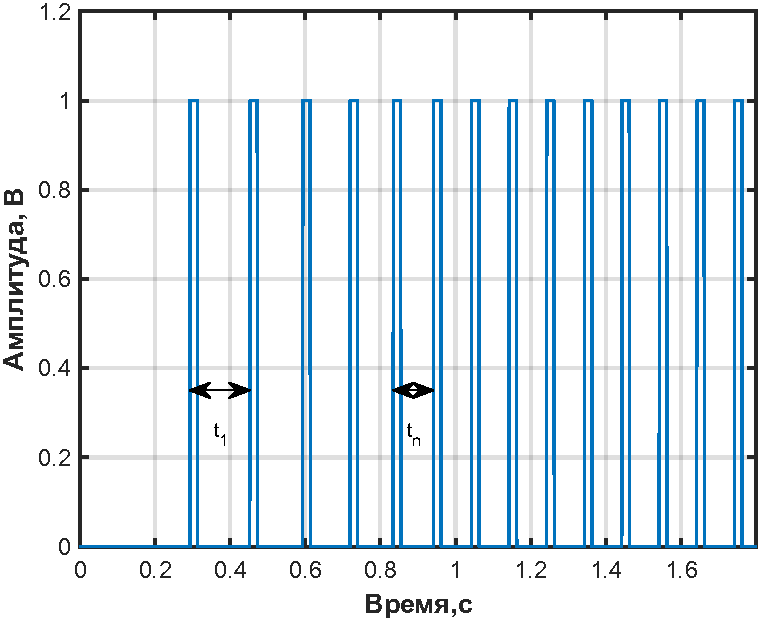
\includegraphics[scale=1]{matlab/img/encoder.pdf} 
	}
	\caption{Осциллограмма сигнала преобразователя угловых перемещений}
	\label{fig:encoder} 
\end{figure}

Угловое ускорение определяется так:

\begin{equation}
	\label{eq:flyweel_acc}
	\varepsilon = \frac{\omega_k-\omega_1}{t_k-t_1}
\end{equation}

где \(\omega_1, \omega_k\) --- начальная и конечная угловая скорость на участке разгона, \(t_1, t_k\) --- соответствующие моменты времени.

\subsection{Оценка бюджета погрешности}

Полный бюджет неопределённости формируется через разложение всех источников ошибок и последующее вычисление их вклада в итоговую величину измеряемого тестового момента.

\subsubsection{Погрешность момента инерции}

\subsubsection{Погрешность ускорения}

Угловое ускорение $\varepsilon_m$ определяется через приращение угловой скорости за интервал времени $\Delta T$.

\begin{equation}
	\label{eq:acc_err}
	\varepsilon_m=\frac{\omega_k-\omega_1}{\Delta T} \quad \quad \omega = \frac{2 \pi}{\Delta t}
\end{equation}

Погрешность угла -- паспортная характеристика углового преобразователя -$\pm 10^{\prime\prime}$. При стандартном распределении это соответствует неопределённости:

\begin{equation}
	\label{eq:u_thtta}
	u_\theta = \frac{10}{\sqrt{3}} \approx \SI{2,8e-5}{\radian}
\end{equation}

Эта погрешность проявляется как разброс временного положения метки:

\begin{equation}
	\label{eq:u)_theta_t}
	u_{t, \theta} = \frac{u_\theta}{\omega}
\end{equation}

Интервал времени $\Delta t$ фиксируется по осциллографу TDS1012B. Для равномерного распределения в пределах шага квантования $q$ стандартная неопределённость равна

\begin{equation}
	\label{eq:u_t,clk}
	u_{t,clk}=\frac{u}{\sqrt{12}}
\end{equation}

Совместная неопределённость измеренного интервала:

\begin{equation}
	\label{eq:u_dt}
u_{\Delta t}
= \sqrt{\,u_{t,\mathrm{clk}}^{\,2}
	+ \left(\frac{\sqrt{2}\,u_{\theta}}{\omega}\right)^{2}}
	\end{equation}
	
	
\section{Измерение реактивного момента оптико-механической системы}

После установки изделия в изделиедержатель подвесная система переводится в состояние покоя. Для этого фиксируют платформу в исходном положении и ожидают затухания переходных процессов до уровня, при котором остаточные колебания не превышают допустимой амплитуды (менее 1 \% от рабочего сигнала гироскопа).

Задаётся эталонный момент с помощью тестового маховика. Скорость колебаний регистрируется гироскопом с частотой дискретизации $f_s=\SI{100}{\hertz}$. Для уменьшения случайных составляющих, измерения повторяются 10 раз.
График скорости колебаний стенда представлен на рисунке \cref{fig:flyweel_stand_spd}
Усреднённый массив угловой скорости вычисляется по формуле:

\begin{equation}
	\label{eq:mean_spd}
	\overline{\omega_{i}}=\frac{1}{N}\sum_{j=1}^{N}\omega_{i}^{(j)}, \qquad N = 10.
\end{equation}

где \(\omega_{i}^j\) --- значение угловой скорости в $i-$ой точке при $j-$ом повторе.

Из усреднённого массива вычисляется угловое ускорение методом численного дифференцирования:

\begin{equation}
	\label{eq:mean_acc}
	\varepsilon_{i}
	= \frac{\overline{\omega}_{i+1}-\overline{\omega}_{i}}{\Delta t},
	\qquad
	\Delta t = \frac{1}{f_s}.
\end{equation}

На участке равноускоренного движения определяется среднее значение ускорения:


\begin{equation}
	\label{eq:acc}
	\varepsilon_m = \frac{1}{n}\sum_{i=1}^{n} \varepsilon_{i}
\end{equation}

где \(n\) --- число отсчётов на участке равномерного ускорения.

После задания эталонного момента выполняется измерение реактивного момента исследуемой ОМС. Привод изделия осуществляет поворот подвижной части на заданный угол. Под действием реактивного момента подвес совершает колебания, скорость которых  регистрирует гироскоп.

Данные обрабатываются аналогично: формируется усреднённый массив скорости колебаний:

\begin{equation}
	\label{eq:omega_op}
	\overline{\omega_{o,i}}
	= \frac{1}{N}\sum_{j=1}^{N} \omega_{o,i}^{(j)}
\end{equation}

После выполняется численное дифференцирование:

\begin{equation}
	\label{eq:epsilon_op}
	\varepsilon_{o,i}
	= \frac{\overline{\omega}_{o,\,i+1}
		- \overline{\omega}_{o,\,i}}{\Delta t}\
\end{equation}

Среднее ускорение на равноускоренном участке находится как:

\begin{equation}
	\label{eq:epsilon_op_mean}
	\varepsilon_{o}
	= \frac{1}{n}\sum_{i=1}^{n} \varepsilon_{o,i}\,.
\end{equation}

Искомый остаточный реактивный момент рассчитывается через соотношение:

\begin{equation}
	\label{eq:Mom}
	M_o = M_m \cdot \frac{\varepsilon_o}{\varepsilon_m}
\end{equation}

Окончательное значение реактивного момента определяется как максимальное по модулю среди положительного и отрицательного экстремумов:

\begin{equation}
	\label{eq:Mom}
	M_{max} = max\{|M^+|, |M^-|\}
\end{equation}



\section{Метрологическая аттестация стенда}

Разработанный стенд прошёл метрологическую аттестацию в установленном порядке. 
Аттестация выполнена АО «НПО Техномаш» имени С.~А.~Афанасьева при поддержке 
Госкорпорации «Роскосмос». По результатам процедуры выдано свидетельство 
№~030-500/2024-61 (РОСС RU.0001.310066/2024), зарегистрированное в государственном 
реестре под номером ФР.1.28.2024.49055.

Методика измерения некомпенсированного возмущающего момента признана 
соответствующей требованиям ГОСТ~Р~8.563--2009. Диапазон измеряемых значений 
составляет от $10^{-3}$ до $1 \,\text{Н}\cdot\text{м}$.  

Погрешность метода оценивалась при измерении момента 
$M = 0{,}005 \,\text{Н}\cdot\text{м}$ и составила:
\[
\delta M = \frac{7{,}07 \cdot 10^{-5}}{0{,}005} \approx 1{,}5 \,\%.
\]

Таким образом, стенд обеспечивает требуемую точность измерений 
и может быть использован в качестве средства поверки и исследований 
оптико-механических систем.

\section{Метрологическая аттестация стенда}

Разработанный стенд прошёл метрологическую аттестацию в установленном порядке. 
Аттестация выполнена АО «НПО Техномаш» имени С.~А.~Афанасьева при поддержке 
Госкорпорации «Роскосмос». По результатам процедуры выдано свидетельство 
№~030-500/2024-61 (РОСС RU.0001.310066/2024), зарегистрированное в государственном 
реестре под номером ФР.1.28.2024.49055.

Методика измерения некомпенсированного возмущающего момента признана 
соответствующей требованиям ГОСТ~Р~8.563--2009. Диапазон измеряемых значений 
составляет от $10^{-3}$ до $1 \,\text{Н}\cdot\text{м}$.  

Погрешность метода оценивалась при измерении момента 
$M = 0{,}005 \,\text{Н}\cdot\text{м}$ и составила:
\[
M = 0,005 \pm \SI{7,07e-5}{\newton\meter} 
\]
\[
\delta M = \frac{7{,}07 \cdot 10^{-5}}{0{,}005} \approx 1{,}5 \,\%.
\]

Таким образом, стенд обеспечивает требуемую точность измерений 
и может быть использован в качестве средства поверки и исследований 
оптико-механических систем. Сертификат аттестации представлен в приложении ~\cref{app:certificate}


\section*{Выводы по главе}

В данной главе разработан и создан испытательный стенд для измерения остаточных реактивных моментов оптико-механических систем.  
Построена теоретическая модель стенда в виде колебательного звена, что позволило определить требования к собственным частотам и декременту затухания подвесной системы. На основе анализа выбрана конструкция со струной в качестве упругого элемента, обеспечивающая малый уровень диссипативных потерь и одну степень свободы для исследуемого изделия.

Стенд оснащён волоконно-оптическим гироскопом для регистрации угловых колебаний и тестовым маховиком с известным моментом инерции для формирования эталонного воздействия. Разработана методика измерений, включающая юстировку подвесной системы, контроль климатических параметров и процедуры определения тестового момента. Проведена оценка бюджета погрешности, показавшая, что основными источниками неопределённости являются точность задания углового ускорения и погрешность измерения момента инерции маховика.

Созданный комплекс прошёл метрологическую аттестацию в установленном порядке, что подтверждает его пригодность для практического применения. Диапазон измеряемых значений составил от $10^{-3}$ до $1 \,\text{Н}\cdot\text{м}$ при относительной погрешности не более 1,5 \%. Это обеспечивает возможность достоверного определения остаточных реактивных моментов при испытаниях оптико-механических систем.

Таким образом, в работе сформирован базис для последующих экспериментальных исследований влияния реактивных моментов на смаз и качество изображений. 



\clearpage
